\section{Introduction}\label{s:intro}

% Abstract
This chapter considers the problem of obtaining dense 3D reconstructions of articulated subjects from single and partially occluded views. Humans generally have no problem in predicting, at least approximately, the 3D structure of most scenes including the pose and shape of animals or other people, even from a single view.
However, the visual evidence available in a single 2D image notoriously~\citep{Faugeras01geometry} contains insufficient information for the third dimension to be recovered uniquely. 
This chapter follows a growing body of work that views 3D reconstruction of articulated subjects in a probabilistic setting, and proposes that the goal of reconstruction methods should be to make the posterior distribution as sharp as possible by learning an strong prior over the space of possible solutions. 
In particular, the method described in this chapter recovers \emph{several} plausible and diverse 3D reconstructions which are compatible with the input data. This is implemented using a novel multi-hypothesis neural network architecture, trained using a best-of-$M$ loss where each of the $M$ hypotheses is constrained to lie on a manifold of plausible poses by means of a generative model. Various improvements are suggested to the standard best-of-$M$ setup, to produce reconstruction sets of an arbitrary size, ensuring these are plausible and diverse by means of a learnt normalizing flow prior and discouraging mode degeneration with a multi-hypothesis reprojection loss.
A fundamental insight is that ambiguities in 3D body poses can be effectively modelled using a similar parameterization as in previous chapters, using a suitable 3D morphable model.
As well as being the first system capable of modelling ambiguities in 3D animal reconstruction, the method is shown to outperform alternative approaches in ambiguous pose recovery on standard benchmarks for 3D humans and in heavily occluded versions of these benchmarks. The chapter begins by introducing key concepts relied upon in this chapter as well as related literature, followed by a description of the method, an evaluation section and finishes with conclusions and opportunities for future work.

\begin{figure}
\setlength{\fboxsep}{0pt}%
\setlength{\fboxrule}{0pt}%
\centering{\begin{tabular}{@{}c@{}}
    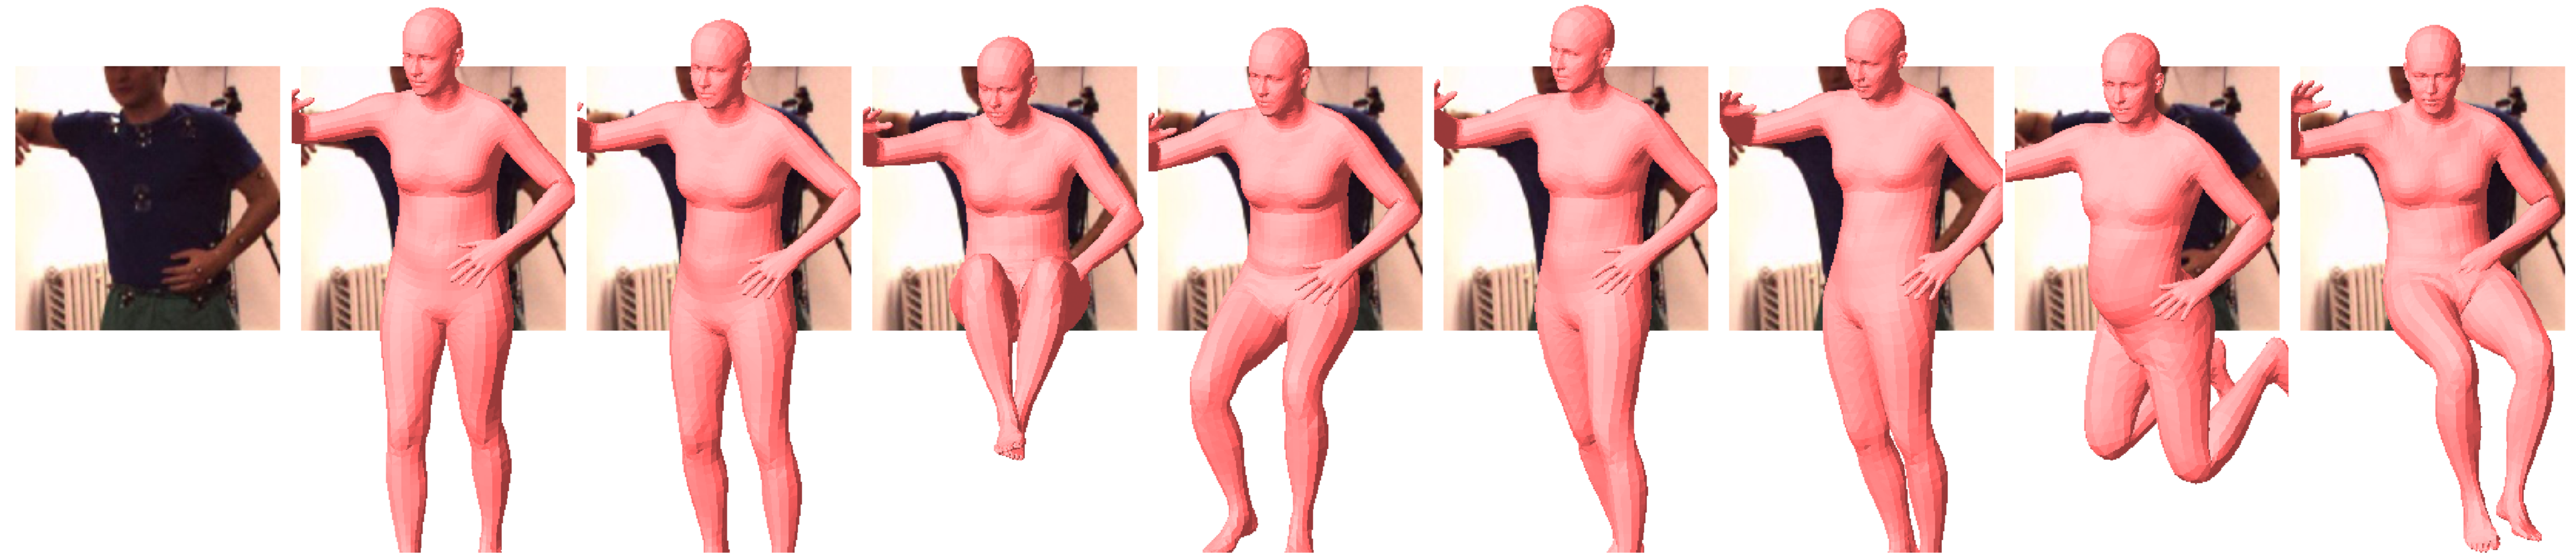
\includegraphics[width=0.49\linewidth,trim=4 8 8 10,clip]{splash/sample_2.pdf} 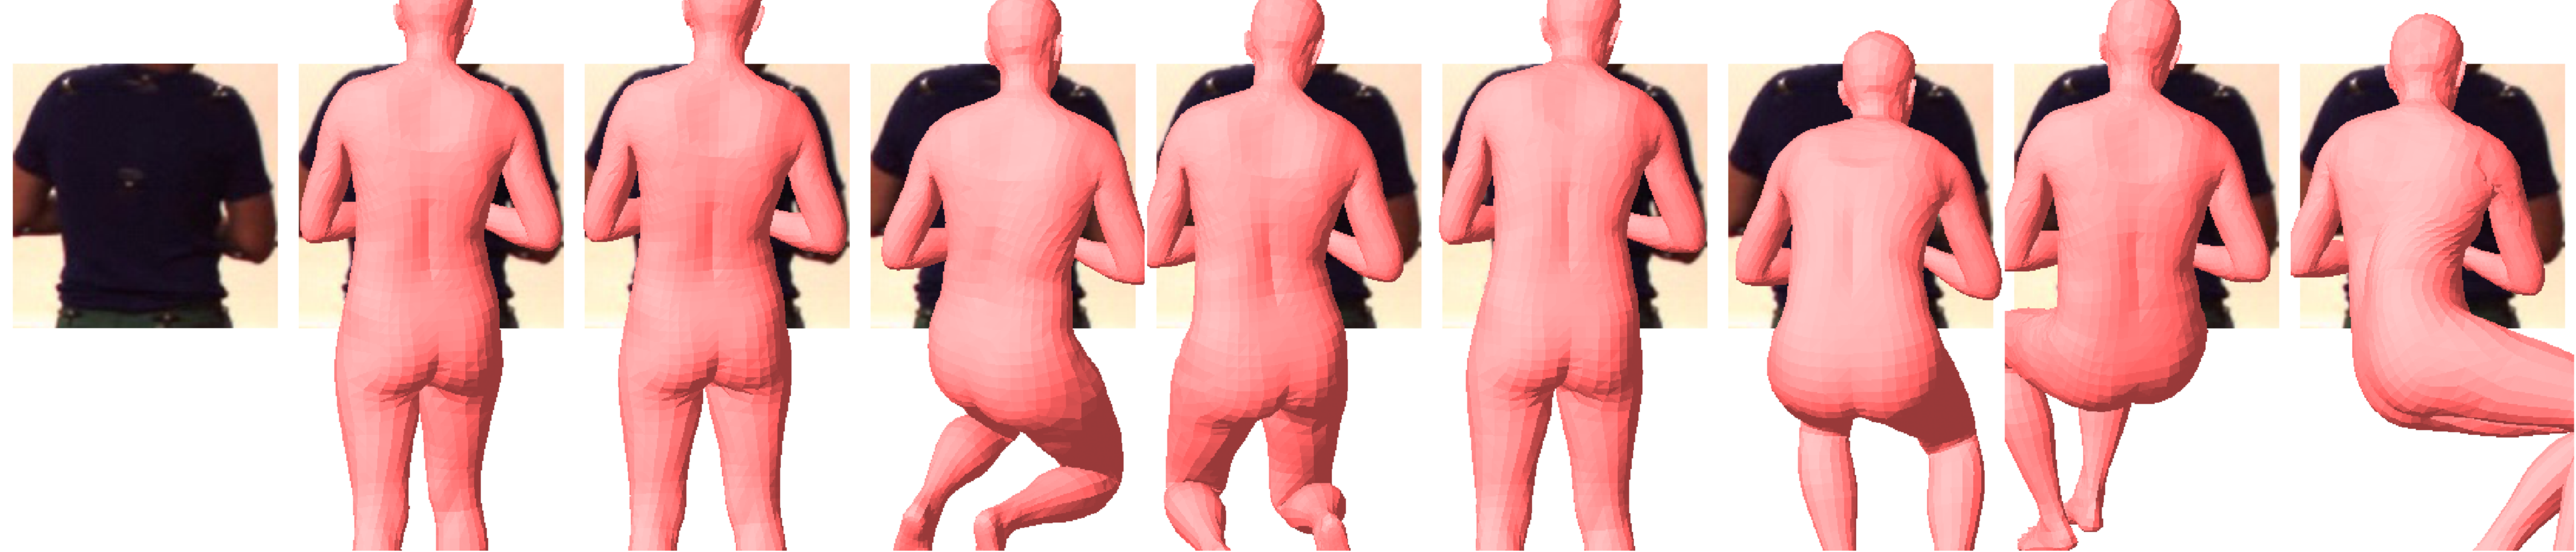
\includegraphics[width=0.49\linewidth,trim=4 8 8 10,clip]{splash/sample_7.pdf}\\
    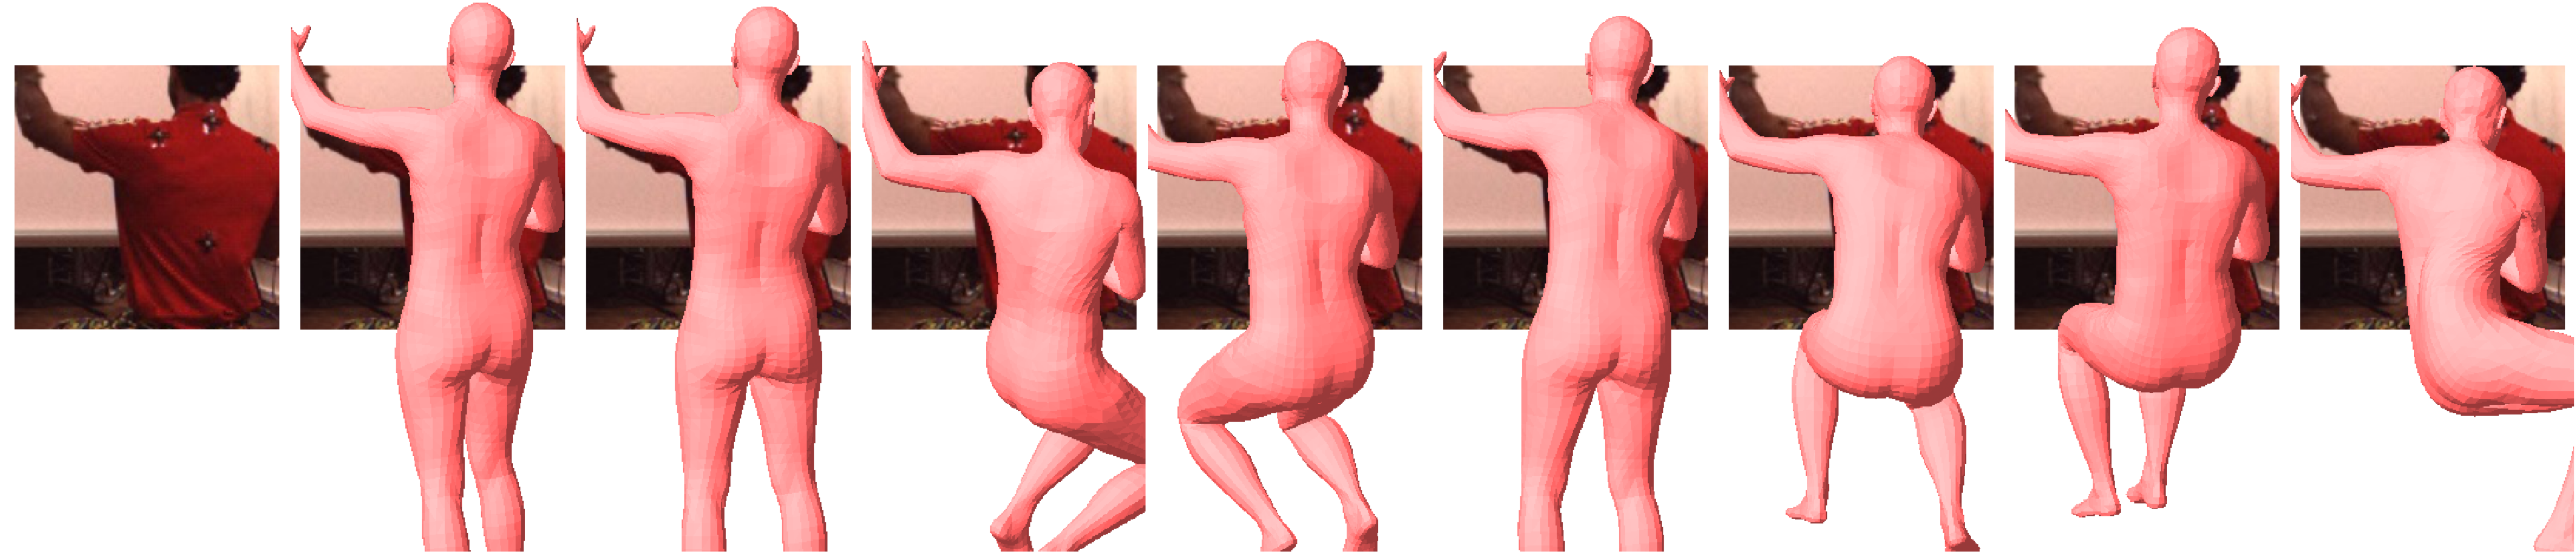
\includegraphics[width=0.49\linewidth,trim=8 10 10 12,clip]{splash/sample_8.pdf} 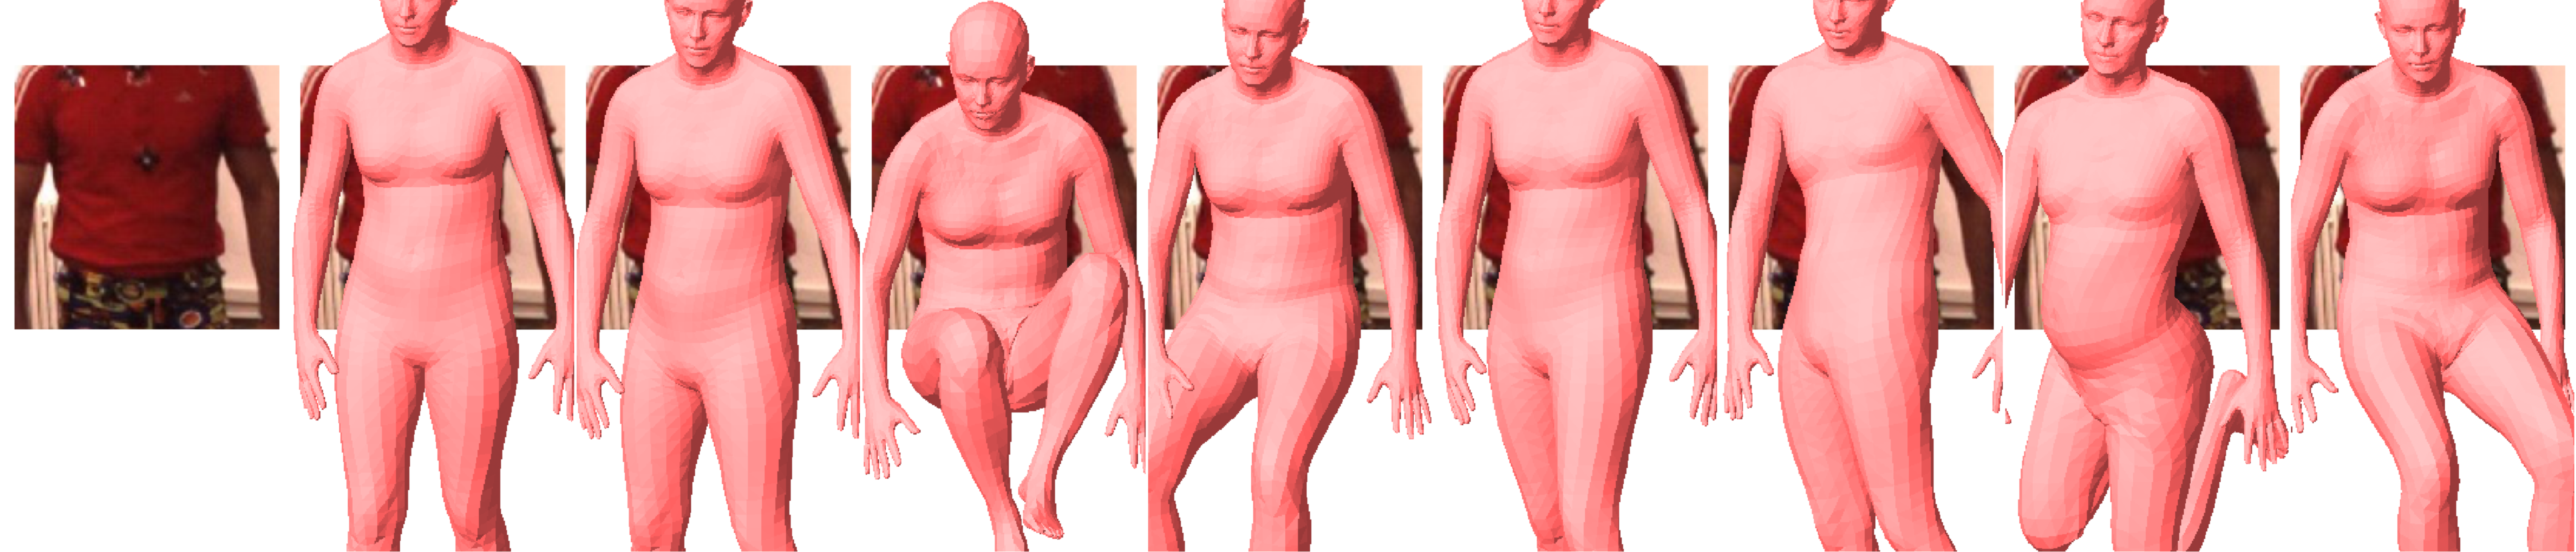
\includegraphics[width=0.49\linewidth,trim=8 10 10  10,clip]{splash/sample_13.pdf}
\end{tabular}}
\captionof{figure}{
\textbf{Human mesh recovery in an ambiguous setting.}
We propose a novel method that, given an occluded input image of a person, outputs the set of meshes which constitute plausible human bodies that are consistent with the partial view.
The ambiguous poses are predicted using a novel $n$-quantized-best-of-$M$ method.\label{fig:splash}}
\end{figure}


\subsection{Limitations of state-of-the-art 3D reconstruction techniques}

As discussed in~\Cref{chap:relwork}, recent progress in single-view 3D model reconstruction for articulated subjects has been impressive.
Methods such as 3D-Safari~\cite{xxx} and \Cref{chap:wldo} of this thesis for animals and HMR~\cite{kanazawa18end-to-end}, GraphCMR~\cite{kolotouros19convolutional} and SPIN~\cite{kolotouros19learning} for humans, formulate the task using a deep neural network that maps 2D images to the parameters of a 3D morphable model (usually SMAL~\cite{zuffi2017menagerie} for animals and SMPL~\cite{loper15smpl} for humans).
Although these methods work well in general, they are not immune from failure cases~(\Cref{fig:issues}).
Their main weakness is when processing \emph{heavily occluded images} of the subject.
When a large part of the subject is missing, say the hind legs of an animal or lower body of a sitting human, they output reconstructions that are often implausible.
Since these approaches produce only one hypothesis as output, they very likely learn to approximate the mean of the posterior distribution, which may not correspond to any plausible pose.
This can be understood with a simple thought experiment. Consider an agent which must randomly choose to travel left or right to avoid an oncoming lake. If the agent applies a policy to average these two possibilities, it will lead the agent to travel straight forwards, realising a suboptimal outcome of travelling straight into the lake.
Unfortunately, the failure modality caused by ambiguous imagery is rather common in animal and human scenes due to environmental and self-occlusion, due to environmental clutter and crowds.

% Discuss other approaches for dealing with this limitation
This chapter proposes a system that handles these existing limitations. The approach recovers 3D mesh reconstructions of complex articulated objects such as animals or humans from highly ambiguous image data, often containing significant occlusions of the object.
Clearly, it is generally impossible to reconstruct the object uniquely if too much evidence is missing; however, it is still possible to predict a \emph{set} containing all possible reconstructions (see \Cref{fig:splash}).
While ambiguous pose reconstruction has been previously investigated, this work proposes the first deep learning approach for ambiguous reconstructions of the \emph{full articulated mesh}.

\begin{figure}[t]
    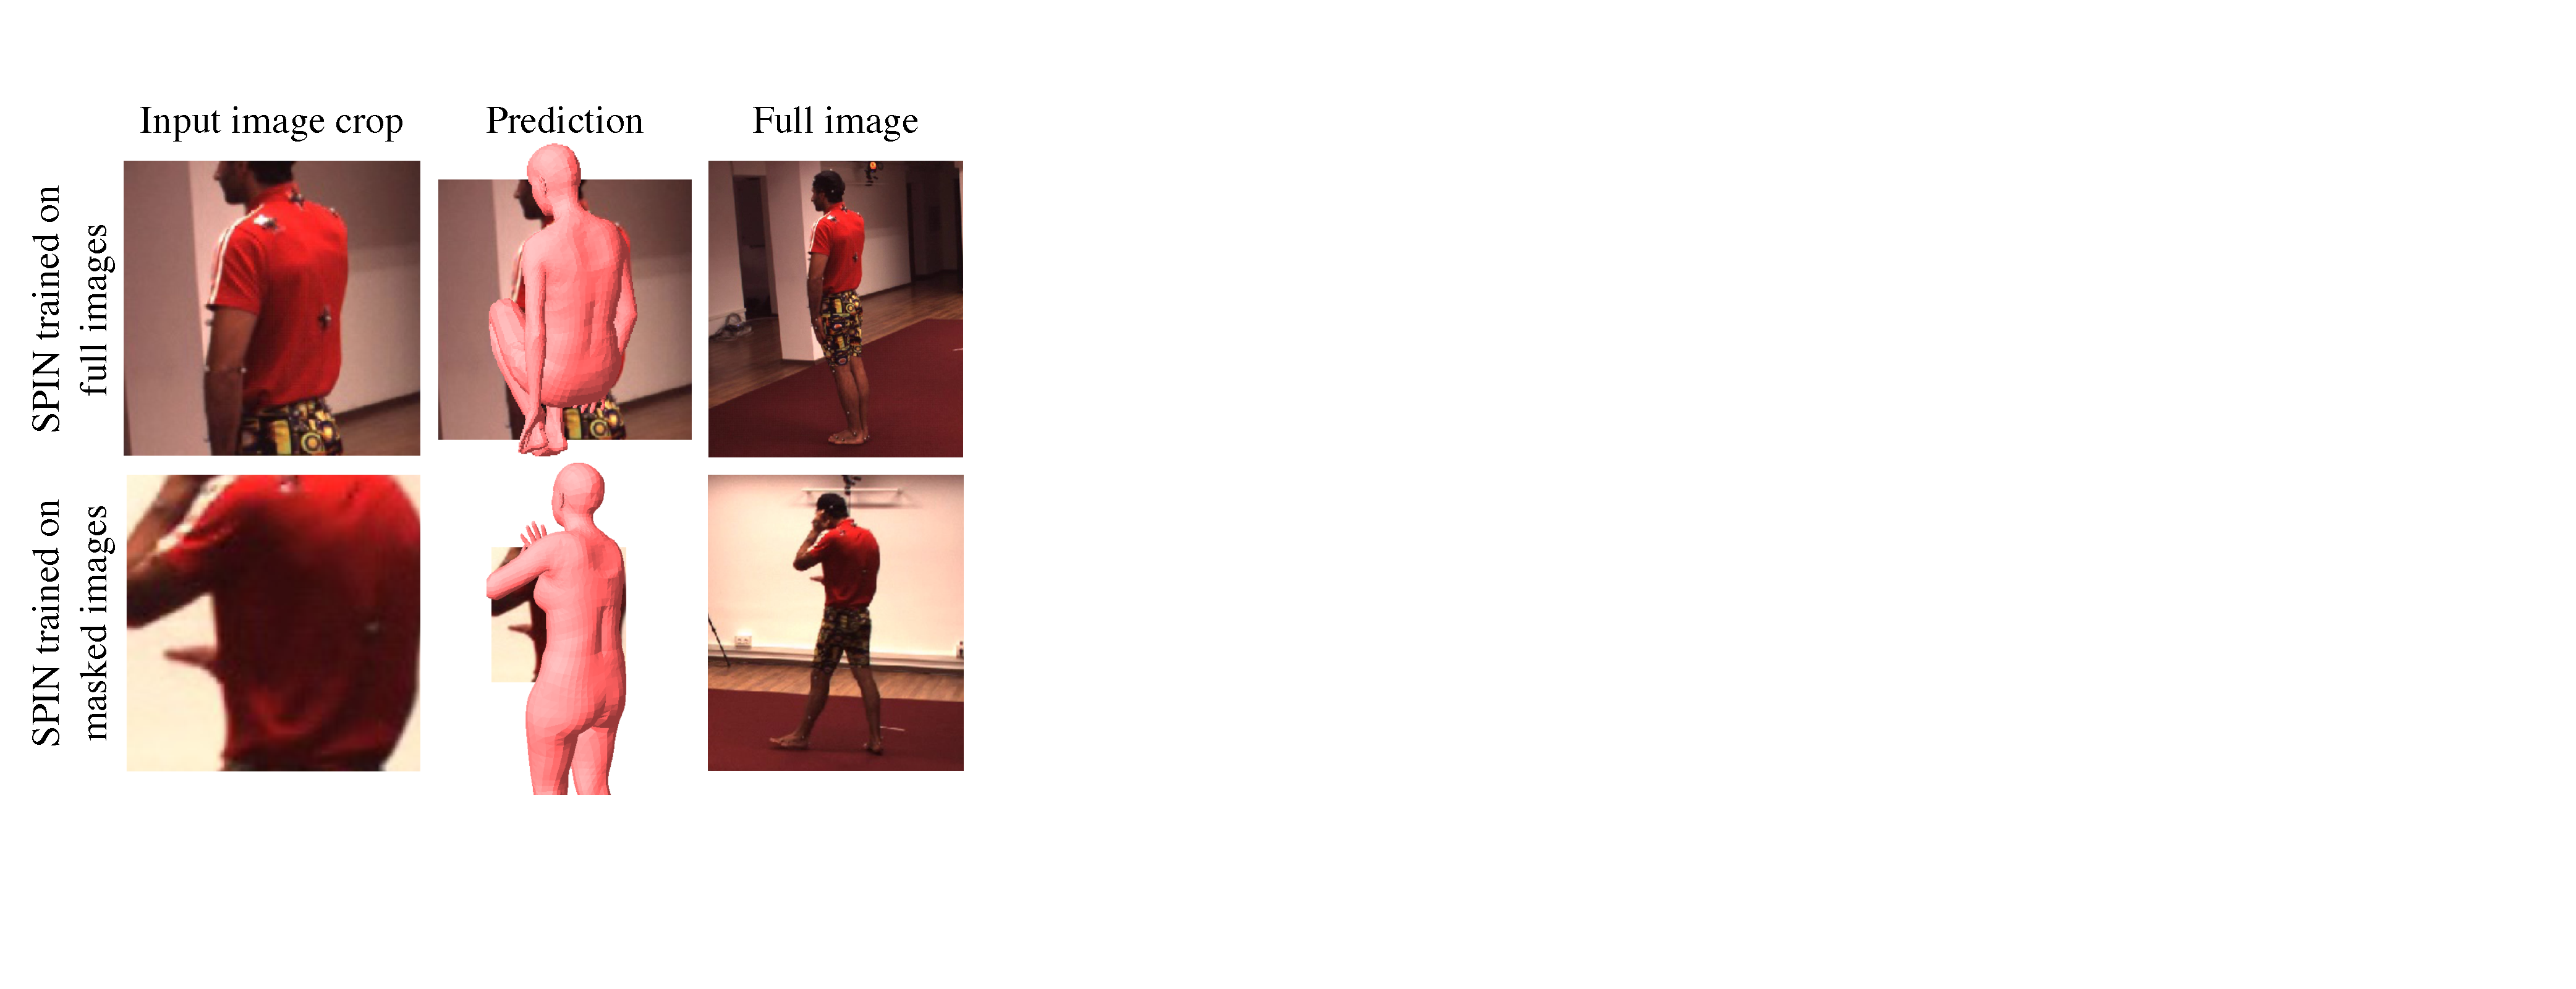
\includegraphics[width=\linewidth]{failures/failure_summary_v2} %
    \caption{
        \textbf{Top}: Pretrained SPIN model tested on an ambiguous example, \textbf{Bottom}: SPIN model after fine-tuning to ambiguous examples. Note the network tends to regress to the mean over plausible poses, shown by predicting the missing legs vertically downward --- arguably the average position over the training dataset.}\label{fig:issues}
\end{figure}


\subsection{Modelling ambiguities in 3D reconstruction}

% kinematic-jump-processes http://www.cs.toronto.edu/~crismin/PAPERS/kinematic.pdf
% tracking-3d-human-figures http://luthuli.cs.uiuc.edu/~daf/courses/AppCV/Papers-2/eccv00.pdf
% desity-prop https://citeseerx.ist.psu.edu/viewdoc/download?doi=10.1.1.119.1950&rep=rep1&type=pdf
% akhter15pose-conditioned https://openaccess.thecvf.com/content_cvpr_2015/papers/Akhter_Pose-Conditioned_Joint_Angle_2015_CVPR_paper.pdf
% ligenerating https://openaccess.thecvf.com/content_CVPR_2019/papers/Li_Generating_Multiple_Hypotheses_for_3D_Human_Pose_Estimation_With_Mixture_CVPR_2019_paper.pdf
% bishop94mixture https://publications.aston.ac.uk/id/eprint/373/1/NCRG_94_004.pdf
% sharma19monocular https://openaccess.thecvf.com/content_ICCV_2019/papers/Sharma_Monocular_3D_Human_Pose_Estimation_by_Generation_and_Ordinal_Ranking_ICCV_2019_paper.pdf
% cheng19occlusion-aware https://openaccess.thecvf.com/content_ICCV_2019/papers/Cheng_Occlusion-Aware_Networks_for_3D_Human_Pose_Estimation_in_Video_ICCV_2019_paper.pdf

% rupprecht17learning: learning in an uncertain world: https://arxiv.org/pdf/1612.00197.pdf

% Resolving 3D https://arxiv.org/abs/1908.06963

% https://arxiv.org/abs/1807.01511 (deep autoencoder)


Several previous papers have looked at the problem of modelling ambiguous 3D human pose reconstructions. Early work includes~\cite{kinematic-jump-processes} who rely on known body segement lengths to resolve depth ambiguities at each joint. Sidenbldh et al.~\cite{tracking-3d-human-figures} define a probalistic method for tracking 3D articulated humans based on a prior probabilisty distribution over pose that models how humans are expected to move. Sminchisescu et al.~\cite{density-prop} describe a mixture density propagation algorithm for predicts the conditional state distributon necessary for 3D body pose tracking based on input silhouettes. More recently, ~\cite{cheng19occlusion-aware} tackle the problem of video 3D reconstruction in the presence of occlusions, and show that temporal cues can be used to disambiguate the solution. 
% While our method is similar in the goal of correctly handling the prediction uncertainty, we differ by applying our method to predicting \emph{full mesh} of the human body.
% This is arguably a more challenging scenario due to the increased complexity of the desired 3D shape.

% The method is similar in that it attempts to handle prediction uncertainty, although the work in this chapter differs by predicting the \emph{full mesh} of the subject. This is arguably a more challenging scenario due to the increased complexity of the desired 3D shape.


The following paragraphs describe implementations of common approaches used to model prediction uncertainty in deep networks. Note that the methods discussed, including Mixture Density Networks~\cite{bishop94mixture,li19generating} and Conditional Variational Auto-Encoders~\cite{sharma19monocular} differ from the work in this chapter as they output a distribution over reconstructed \emph{3D locations} of a finite set of human body joints, rather than a full mesh. This chapter argues that the parameters of a 3D morphable model offers a better space for coding not just 3D shapes and poses, but also their ambiguities. In addition, predicting a full mesh is a more challenging scenario due to the increased complexity of the desired 3D shape. A later section in this chapter describes how these techniques can be extended to act as baselines for the system proposed here. 
% TODO: An exception is the very recent work of BLAH, who extend the ar

% As far as we could determine, the work in this chapter is the first to model ambiguous reconstructions directly in the space of human body model parameters, although notable works such as ~\cite{xxx} have come later and are worthy of discussion.
% Ignas paper

% To be fair, we don't learn a prior directly on the SMPL parameters.

% They model distributions conditioned on the parent of each joint in the kinematic tree and show that this prior can be used to obtain improved parametric fits.
% More recently,~\citet{akhter15pose-conditioned} estimate a 3D human stick figure from 2D joint locations, making use of a prior over joint angles learnt from a motion capture dataset.

\subsubsection{Mixture Density Networks (MDN)}

Li et al. ~\cite{li19generating} use the Mixture Density Networks model of~\cite{bishop94mixture} to capture ambiguous 3D reconstructions of sparse human body keypoints (rather than a full mesh as in this work) directly in physical space. 

The idea of a Mixture Density Network for articulated 3D reconstruction is to represent the probability of a 3D pose vector $x \in \R{3N}$ given an input set of features $y \in \R{M}$. $y$ is left general here, but could be for example a set of 2D keypoints, extracted image features etc. $w$ are the neural network weights. The posterior density is given as a linear combination of $M$ Gaussian functions
\begin{equation}
  p(x | y, w) = \sum_{i}^{M} \Pi_{i}(y, w)\phi_{i}(x | y, w)
\end{equation}

Here, $\Pi_{i}(y, w)$ are mixing coefficients which must satisfy $0 \leq \Pi_{i}(y) \leq 1$ and $\sum_{i=1}^{M} = 1$. $\phi(x | y, w)$ is the conditional distribution of the 3D pose $x$ for the $i^{th}$ Gaussian component. 

\begin{equation}
  \phi(x | y, w) = 
    \frac{
      1
    }{
      (2\pi)^{\frac{d}{2}} \sigma_{i}(y, w)^{d}
    } 
    \exp{
    -\frac{
      || x - \mu_{i}(y, w) ||^{2}
    }{
      2\sigma_{i}(y, w)^{2}
    }
  }
\end{equation}

A dataset of $K$ independent and identically distributed training examples including input $X$ and 3D poses $Y$ can be used to optimize the weights $w$ of such a network. The posterior distribution of $w$ is given by

\begin{align}
  p(w | X, Y) 
  &\propto p(X | Y, w)p(w, Y) \\
  &= p(w | Y) \prod_{j=1}^{K} p(x_j | y_j, w)
  % &= p(w | X) \prod_{j=1}^{K} \sum_{i=1}^{M} \Pi_{i}(x_{j}, w) \phi_{i} (y_{j} | x_{j}, w)
\end{align}

The optimal weight $w^{*}$ is obtained by minimizing the negative log-posterior

\begin{align}
  w^{*} &= \argmin_{w} -\log p(w | X, Y) \\
        &= \argmin_{w} \left[-\sum_{j=1}^{K} \log p(x_j | y_j, w)\right] - \log p(w | Y)
\end{align}

This formulation can be used to form a loss function to optimize the network. 

\begin{equation}
  L = \left[-\sum_{j=1}^{K} \log p(x_j | y_j, w)\right] - \log p(w | Y)
\end{equation}

This can be deconstructed into two terms, $L = L_{3D} + L_{PRIOR}$. $L_{3D}$ tunes the network weights such that ground truth 3D poses are likely under the model, and $L_{PRIOR}$ which acts as a prior over $\mu(w, Y), \sigma(w, Y)$ and $\Pi(w, Y)$. In the Li et al.~\cite{xxx} implementation, the prior is uniform over $\mu(w, Y)$ and $\sigma(w, Y)$, and a Dirichlet~\cite{xxx} conjugate prior is used over the mixture coefficients $\Pi(w, Y)$. 

For completeness, the 3D alignment term is given as
\begin{equation}
  L_{3D} = -\sum_{j=1}^{K} \log \sum_{i=1}^{M} \Pi_{i}(y_{j}, w) \phi_{i}(x_j | y_j, w)
\end{equation}

% https://arxiv.org/pdf/2103.10978.pdf
A version of this setup is used as a baseline in the later experiment section, although adapted to model the conditional probability of 3D morphable model joint angles through the generator function. Another notable work in this category (released after the content of this chapter) is that of Sengupta et al~\lazycite{Sengupta}{} who extend the MDN formulation to model ambiguity in pose and shape, operating on a collection of human images. 

\subsubsection{Conditional Variational Auto-Encoder (CVAE)}

Another approach, proposed by \citet{sharma19monocular} is to learn a conditional variational auto-encoder (CVAE) to model ambiguous reconstructions as a posterior distribution. 

To explain this, first consider a simple directed, latent variable model. $x$ is the observed variable, and $u$ is a latent variable, or \emph{code}, which should provide information about $x$.

% \begin{center}
% \begin{tikzpicture}
%   \SetGraphUnit{5}
%   \Vertex{x}
%   \WE(x){z}
%   \WE(z){y}
%   \Edge(z)(x)
%   \Edge(y)(z)
%   % \Edge[label = 2](B)(C)
%   % \Edge[label = 3](C)(B)
%   % \Edge[label = 4](B)(A)
%   % \Loop[dist = 4cm, dir = NO, label = 5](A.west)
%   % \Loop[dist = 4cm, dir = SO, label = 6](C.east)
%   % \tikzset{EdgeStyle/.append style = {bend left = 50}}
%   % \Edge[label = 7](A)(C)
%   % \Edge[label = 8](C)(A)
% \end{tikzpicture}
% \end{center}

\begin{center}
  \begin{tikzpicture}
    \SetGraphUnit{5}
    \Vertex{x}
    \WE(x){z}
    \Edge(z)(x)
    % \Edge[label = 2](B)(C)
    % \Edge[label = 3](C)(B)
    % \Edge[label = 4](B)(A)
    % \Loop[dist = 4cm, dir = NO, label = 5](A.west)
    % \Loop[dist = 4cm, dir = SO, label = 6](C.east)
    % \tikzset{EdgeStyle/.append style = {bend left = 50}}
    % \Edge[label = 7](A)(C)
    % \Edge[label = 8](C)(A)
  \end{tikzpicture}
  \end{center}

The joint distribution of such a model is given as

$$
  p_{\theta}(x,z) = p(x|z)p(z)
$$

% $$
%   p_{\theta}(x,z,y) = p(x|z)p(z|y)p(y)
% $$


This type of latent variable model can be viewed as a generative process for obtaining the observed data $x$. The procedure for this is:

% $$
% \begin{aligned}
%   y &\sim p(y) \\
%   z &\sim p(z|y) \\
%   x &\sim p(x|z)
% \end{aligned}
% $$

$$
\begin{aligned}
  z &\sim p(z) \\
  x &\sim p(x|z)
\end{aligned}
$$

This represents sampling a latent vector $z$ from the prior distribution $p(z)$ followed by sampling data $x$ from the conditional likelihood distribution $p(x|z)$. The variational autoencoder comprises a probabilistic encoder $p(z|x)$ that describes the distribution of the latent variables given data, and a probabilistic decoder $p(x|z)$ which describes the distribution of the data given the latent variable. 

% There are two objectives. First, $p$ must be tuned such that the latent model closely matches the true underlying distribution $p_{data}$. Secondly, to infer good values for the latent variables $z$ given observed data, in other words to calculate the posterior $p(z|x)$. 
% p(z|x,y)

Bayes theorem can be used to draw the link between these terms. 
% $$
% \begin{aligned}
%   p(z|x,y) 
%   &= \frac{p(x|y,z)p(z|y)}{p(x|y)} \\
%   &= \frac{p(x|y,z)p(z|y)}{\int p(x|y,z)p(z|y) \,dz}
% \end{aligned}
% $$
$$
\begin{aligned}
  p(z|x) 
  &= \frac{p(x|z)p(z)}{p(x)} \\
  &= \frac{p(x|z)p(z)}{\int p(x|z')p(z') \,dz'}
\end{aligned}
$$

% A simple way to set up terms is to assume $p(z) = \mathcal{N}(0, I)$ is a standard Gaussian distribution and $p(x|z) = \mathcal{N}(f(z),g(z))$ is a Gaussian parameterized by outputs of neural networks $f, g$. 
Unfortunately, $p(z|x)$ is generally intractable for high-dimensional $z$ since the integral is taken over all possible configurations of latent variables $z$ (or $z'$ as in the expansion above). Even estimation attempts based on Monte Carlo tend to fail due to high variance in gradient estimates. % ASK AWF!? Ask why this fails? can't you just try fewer samples? is this because the distribution is very 'isolated'


% $p(x,z,y)$
% The Kullback-Leibler (KL) divergence can be used to measure how closely $p(x,z)$ fits a training dataset. Divergence is measured between the data distribution $p_{data}(x)$ and the model's marginal distribution $p(x) = \int p(x,z) \,dz$. 
%https://jaan.io/what-is-variational-autoencoder-vae-tutorial/




% Note the integral on the demoninator requires expotential time to compute, since it needs to be evaluate all configurations of latent variables. 
% In practice, this expression is generally intractable for high-dimensional $z$ to compute this expression since the integral is taken integration over all possible configurations of latent variables $z$. 
% Even estimation attempts based on Monte Carlo tend to fail due to high variance in gradient estimates. % ASK AWF!? Ask why this fails? can't you just try fewer samples? is this because the distribution is very 'isolated'

% This is equivalent to maximizing the marginal log-likelihood $log p(x)$ over the dataset $D$. 

% $$
% \max_{p} \sum_{x \in D} \log p_{\theta}(x) = \max_{p} \sum_{x \in D} \log \int p_{\theta}(x,z) \,dz
% $$

Instead, a variational method is used to estimate the intractable posterior $p(z|x)$ using a new tractable distribution $q(z)$. To do this, Kullback-Leibler (KL) divergence can be used to measure the difference between two probability distributions. For example, it can be used to measure how closely the approximation $q(z)$ matches the true distribution $p(z|x)$ 
$KL(q_{\lambda}(z) \| p(z|x))$:
% $KL(q_{\lambda}(z|x,y) \| p(z|x,y))$:

The goal is to find the variational parameters for $q$ that minimize the divergence:

\begin{equation}
  q^{*}(z) = \argmin_{\lambda} KL(q(z) \| p(z|x))
\end{equation}

And looking at this term
$$
\begin{aligned}
KL(q(z) \| p(z|x))
  &= KL(q(z) \| p(z|x)) \\
  &= -\sum_{z \sim q(z)} q(z) \log \frac{p(z|x)}{q(z)} \\
  &= -\sum_{z \sim q(z)} q(z) \log \frac{p(x,z)}{q(z)} \frac{1}{p(x)} \\
  &= -\sum_{z \sim q(z)} q(z) \log \left[ \frac{p(x,z)}{q(z)} - \log p(x) \right] \\
  &= -\sum_{z \sim q(z)} q(z) \log \frac{p(x,z)}{q(z)} 
  + \sum_{z \sim q(z)} q(z) \log p(x) \\
  &= -\sum_{z \sim q(z)} q(z) \log \frac{p(x,z)}{q(z)} 
  + \log p(x) \underbrace{\sum_{z \sim q(z)} q(z)}_{=1} \\
\end{aligned}
$$

Notice that rearraging gives the following expression
$$
\begin{aligned}
  \log p(x) = KL(q_{\lambda}(z) \| p(z|x)) 
  + \underbrace{\sum_{z \sim q(z)} q(z) \log \frac{p(x,z)}{q(z)}}_{ELBO}
\end{aligned}
$$

Recall the aim of this exercise is to minimize $KL(q_{\lambda}(z) \| p(z|x))$. Since $x$ is given, $\log p(x)$ is a constant and as KL is non-negative this can be achieved by maximizing the final term, known as the Evidence Lower Bound (ELBO).
$$
\begin{aligned}
  ELBO 
  &= \sum_{z \sim q(z)} q(z) \log \frac{p(x,z)}{q(z)} \\
  &= \sum_{z \sim q(z)} q(z) \log \frac{p(x|z)p(z)}{q(z)} \\
  &= \sum_{z \sim q(z)} q(z) \left[ \log p(x|z) 
  + \log \frac{p(z)}{q(z)} \right] \\
  &= \sum_{z \sim q(z)} q(z) \log p(x|z) 
  + \sum_{z \sim q(z)} q(z) \log \frac{p(z)}{q(z)} \\
  &= E_{z \sim q(z)} \log p(x|z) - KL(q(z) \| p(z))
\end{aligned}
$$

Peering at the two terms, one can think the first term $E_{z \sim q(z)} \log p(x|z)$ as a reconstruction `loss' which promotes $x's$ generated from $z's$ being likely. The second term $KL(q(z) \| p(z))$ is a regularizer that keeps the approximate distribution $q$ close to $p$. Further, note that the tightness of the lower bound is determined by the specific choice of $q$. In particular, the error between the original expression $\log p(x)$ and the ELBO is given by $KL(q(z) || p(z|x))$. The error is zero if these exactly match.



% $$
% \begin{aligned}
%   q^{*}_{\lambda}(z|x) 
%   &= \argmin_{\lambda} KL(q_{\lambda}(z|x) \| p(z|x)) \\
%   &= \argmin_{\lambda} 
%   \mathbb{E}_{z \sim q(z|x)} \left[ \log q_{\lambda}(z|x) \right]
%   -\mathbb{E}_{z \sim q(z|x)} \left[ \log \frac{p(x,z)p(z)}{p(x)} \right] \\
%   &= \argmin_{\lambda} 
%   \mathbb{E}_{z \sim q(z|x)} \left[ \log q_{\lambda}(z|x) \right]
%   -\mathbb{E}_{z \sim q(z|x)} \left[ \log p(z) \right] 
%   -\mathbb{E}_{z \sim q(z|x)} \left[ \log p(x|z) \right] 
%   +\mathbb{E}_{z \sim q(z|x)} \left[ \log p(x) \right] \\
%   &= \argmin_{\lambda} 
%   \mathbb{E}_{z \sim q(z|x)} \left[ \log q_{\lambda}(z|x) \right]
%   -\mathbb{E}_{z \sim q(z|x)} \left[ \log p(x,z) \right] 
%   + \log p(x)
% \end{aligned}
% $$
% % $$
% % \begin{aligned}
% %   q^{*}_{\lambda}(z|x,y) 
% %   &= \argmin_{\lambda} KL(q_{\lambda}(z|x,y) \| p(z|x,y)) \\
% %   &= \argmin_{\lambda} \mathbb{E}_{q} \left[ \log q_{\lambda}(z|x,y) \right]-\mathbb{E}_{q} \left[ \log p(x,z|y) \right] + \log p(x|y)
% % \end{aligned}
% % $$

% Unfortunately, this is again intractable as the evidence term $p(x)$ appears once more. However, note that with this definition

% $$
% \begin{aligned}
%   \log p(x|y) 
%   &= 
%   \mathbb{E}_{q} \left[ \log p(x,z|y) \right]
%   - \mathbb{E}_{q} \left[ \log q_{\lambda}(z|x,y) \right]
%   + KL(q_{\lambda}(z|x,y) \| p(z|x,y)) \\
%   &= 
%   \underbrace{
%     \mathbb{E}_{q} \left[ q_{\lambda}(z|x,y) \log p(x|z,y) \right]
%   - KL(q_{\lambda}(z|x,y) \| p(z|y))}_{ELBO}
%   + KL(q_{\lambda}(z|x,y) \| p(z|x,y))
% \end{aligned}
% $$

% $$
% \begin{aligned}
%   \log p(x) 
%   &= 
%   \mathbb{E}_{q} \left[ \log p(x,z) \right]
%   - \mathbb{E}_{q} \left[ \log q_{\lambda}(z|x) \right]
%   + KL(q_{\lambda}(z|x) \| p(z|x)) \\
%   &= 
%   \underbrace{
%     \mathbb{E}_{q} \left[ q_{\lambda}(z|x) \log p(x|z) \right]
%   - KL(q_{\lambda}(z|x) \| p(z))}_{ELBO}
%   + KL(q_{\lambda}(z|x) \| p(z|x))
% \end{aligned}
% $$

% This expression can be used to derive the Evidence Lower Bound (ELBO) as follows:
% \begin{equation}
%   \log p(x) 
%   \geq \mathbb{E}_{q} \left[ q_{\lambda}(z|x) \log p(x|z) \right]
%   - KL(q_{\lambda}(z|x) \| p_{\theta}(z))
% \end{equation}
% \begin{equation}
%   \log p(x|y) 
%   \geq \mathbb{E}_{q} \left[ q_{\lambda}(z|x,y) \log p(x|z,y) \right]
%   - KL(q_{\lambda}(z|x,y) \| p_{\theta}(z|y))
% \end{equation}



% $$
% \begin{aligned}
%   \log p_{\theta}(x|y) 
%   &= \log \int p_{\theta}(x, z) \,dz \\
%   &= \log \int p_{\theta}(x, z) \frac{q_{\lambda}(z|x,y)}{q_{\lambda}(z|x,y)} \,dz \\
%   &\geq q_{\lambda}(z|x) \log \frac{p_{\theta}(x, z)}{q_{\lambda}(z|x,y)} \,dz \\
%   &=\mathbb{E}_{q_{\lambda}(z|x,y)} \left[ \log \frac{p_{\theta}(x,z)}{q_{\lambda}(z|x,y)} \,dz \right] \\
% \end{aligned}
% $$

% Note that Jensen's inequality is used in the final step. This final expression is known as the Evidence Lower Bound (ELBO). 


% The tightness of the lower bound is determined by the specific choice of $q$. In particular, the error between the original objective $\log p_{\theta}(x)$ and the ELBO is given by $KL(p(z|x) || q(z|x))$. The error is zero if these exactly match.

% A careful choice of $q_{\lambda}(z)$ leads this construction to admit a tractable unbias Monte Carlo estimator:
% \begin{equation}
%   \log p_{\theta}(x) = \frac{1}{k} \sum_{i=1}^{k} \log \frac{p_{\theta}(x, z_{i})}{q_{\lambda}(z_{i}|x)}, \textrm{where } z_{i} \sim q_{\lambda}(z,x)
% \end{equation}

% Or alternatively,
% \begin{align}
%   \log p_{\theta}(x) 
%   &= \int \log \left[ p_{\theta}(x, z) \frac{p_{\theta}(z)}{q_{\lambda}(z|x)} \right] q(z|x) \,dz \\
%   &= \int \log p_{\theta}(x|z)q_{\lambda}(z|x) \,dz - KL(q_{\lambda}(z|x) \| p_{\theta}(z))
% \end{align}

The next question is how to implement such a model using a deep neural network. Here,

\begin{enumerate}
  \item \textbf{Encoder} $q_{\lambda}(z|x) = \mathcal{N}(z | \mu_{\lambda}(x), \Sigma_{\lambda}(x))$ where $(\mu_{\lambda}(x),\Sigma_{\lambda}(x)) = \Phi_{\lambda}(x)$ are computed by an encoder neural network $\Phi$.
  \item \textbf{Decoder} $p_{\theta}(x|z) = \mathcal{N}(x | \mu_{\theta}(z), \Sigma_{\theta}(z))$ where $(\mu_{\theta}(z),\Sigma_{\theta}(z)) = \Psi_{\theta}(z)$ are computed by a decoder neural network $\Psi$.
  \item \textbf{Prior} $p_{\theta}(z)$ is set to a simple fixed distribution (e.g.~std Gaussian) to ensure $KL(q_{\lambda}(z|x) \| p_{\theta}(z))$ is trivial to compute.
  \item We express samples $z = \mu_{\theta}(x) + \Sigma_{\theta}(x)^{-\frac{1}{2}} \epsilon$ where $\epsilon$ is a sample from an std Gaussian, also known as *reparameterization trick*. We also use the shorthand notation $z = \Phi(x) \square \epsilon$ that captures the fact that $\mu_{\theta}(x)$ and $\Sigma_{\theta}(x)$ are estimated by the encoder $\Phi$.
  \end{enumerate}




% disambiguates the problem, The idea is to map the input to a unit Gaussian distribution which represents the space of possible outputs. A controlled version of the ground truth for the input is then used to select a point in the Gaussian, which serves to disambiguate the 

% ground truth is then used  By carefully restricting information flow, the ground truth 3D output is then used to select the correct mode

% represent the space of possible outputs as a normal distribution 
% The idea behind a CVAE is to represent the space of  

% https://github.com/junyanz/BicycleGAN


Sharma et al.~\cite{xxx} adapt this formulation to model 3D skeletons and produce results on Human3.6M and HumanEva-I. They also propose two scoring methods to extract a single 3D reconstruction from the distribution which can be thought of as an alternative mechanism to the weighted quantizer scheme proposed here. There have also techniques~\cite{xxx} which extend these variational methods to generative adversarial netowrks. These are interesting and further reading here is available from xxx. 




% Several previous papers have looked at the problem of modelling ambiguity in 3D human pose reconstruction. Early work includes~\citet{kinematic-jump-processes}, ~\citet{tracking-3d-human-figures} and \citet{density-prop}. More recently, ~\citet{akhter15pose-conditioned} learn a prior over human skeleton joint angles from a MoCap dataset.
% %(but not directly a prior on the SMPL parameters)
% % They model distributions conditioned on the parent of each joint in the kinematic tree and show that this prior can be used to obtain improved parametric fits.
% More recently,~\citet{li19generating} use the Mixture Density Networks model of~\cite{bishop94mixture} to capture ambiguous 3D reconstructions of sparse human body keypoints directly in physical space.
% \citet{sharma19monocular} learn a conditional variational auto-encoder to model ambiguous reconstructions as a posterior distribution; they also propose two scoring methods to extract a single 3D reconstruction from the distribution.



% BicycleGan etc.

\subsubsection{Min-of-$M$}

The idea of Min-of-N frameworks is to view the posterior distribution as a discrete set of $M$ hypotheses. A neural network is trained to produce $M$ hypotheses $\{f^{m}(Y_{i})\}_{m=1}^{M}$, where $Y_{i}$ is an input vector for the $i^{th}$ movie. In the literature, such multiple hypotheses networks are often trained with a so-called \emph{best-of-$M$} loss --- namely, during training, the loss is incurred only by the best of the $M$ hypothesis, back-propagating gradients from that alone~\cite{guzman2012multiple}. For example, with ground truth 3D points $X_{i}$ the min-of-$M$ loss is given as
\begin{equation}
  \mathcal{L}_\text{best}(Y;m^*)
  =
  \frac{1}{N}
  \sum_{i=1}^N
  \big \| X_{i} - f^{m_i^*}(Y_{i}) \big \|,
  ~~
  m_i^*
  =
  \operatornamewithlimits{argmin}_{m=1,\dots,M}
  \big \| X_{i} -  f^{m}(Y_{i}) \big \|,
\end{equation}

Note that this formulation can be seen as a variant of the mixture density networks as defined previously. In particular, consider an MDN with $M$ modes and reduce the covariance of each Gaussian to a single point. Further analysis of this model is left to the later method section.

This chapter opts for the \emph{best-of-$M$} approach since it has been show to outperform  alternatives (such as variational auto-encoders or mixture density networks) in tasks that are similar to our 3D human pose recovery, and which have constrained output spaces. For example, Rupprecht et al.~\cite{rupprecht17learning} demonstrate the model on classicly ambiguous tasks including human pose estimation and future prediction. The primary contribution in this chapter is the introduction of a principled multi-hypothesis framework which models ambiguities in monocular pose recovery.

% WORKS THAT USE MDNs
%% https://arxiv.org/abs/1807.01511 (deep autoencoder

% \subsubsection{Notes}

% % https://wiseodd.github.io/techblog/2016/12/10/variational-autoencoder/

% To generate the required parameters, we use a 2 stage multi-layer perceptron (MLP) $G: X \mapsto (z, \beta, \gamma, s, t)^{M}$ to generate a latent code $z_{i}$ that can be passed through the inverse flow to generate joint angles $\theta = F^{-1}(z_{i})$, and the remaining components: $\beta_{i}, \gamma_{i}$ and orthographic camera parameters $s_{i}, t_{i}$.

% Once these $M$ SMPL parameterizations have been computed, we can then generate the $M$ meshes using the standard SMPL skinning pipeline:

% $P_{i} = S((\theta_{i}, \beta_{i}, \gamma_{i})$

% We make use of a standard joint regressor $J: K \mapsto \mathbb{R}^{16\times 2}$ in order to compute the approximate 3D joint positions $K \in \mathbb{R}^{16\times 2}$ associated with the input 2D joints. Orthographic projection $\pi(s, t): \mathbb{R}^{16\times 3} \mapsto \mathbb{R}^{16\times 2}$ is then used to generate the predicted set of 2D points.
% From these diverse modes, we apply a loss to ensure they are all consistent with respect to the input set of 2D joints:

% \begin{equation}
%     L_{reproj-input} = \sum_i{|| \pi(s_{i}, t_{i})[J(P_{i})] - x||}
% \end{equation}

% We then apply a 3D joint loss in order to identify the best hypothesis among predicted modes:

% % i* = argmin_{i}{{J(Y_{i})} - y}

% \begin{equation}
%     L_{obj} = L_{joint3d} + L_{reproj-gt} + L_{vertex}
% \end{equation}

% Where

% This, and this and this are the equations.

% We consider the problem of reconstructing $x$ (3D object) form a partial observation $y$ (2D projection).
% We also assume that observations are noisy, so the observation process is described by a known conditional distribution $p(y|x)$.
% We assume that $x$ has a ``useful'' parameterization or code $z$.
% The parameterization is another random variable linked to $x$ via distribution $p(x|z)$.
% While this could be learned, we assume a parameterization is given to us (e.g. SMPL).

% The goal is to: 1) learn an ``inverse function'' $q(z|x)$ inverting the parameterization of the data $x$ and 2) learn a ``prediction'' function $q(z|y)$ that recovers $x$ in code space.
% The assumption is that expressing reconstruction ambiguities is easy in code space, so that $q(z|y)$ is far simple to model than $p(x|y)$; however, we pay the price of having to learn $q(z|x)$.

% We formulate this similar to a conditional variational autoencoder (cVAE):

% $$
% \begin{aligned}
% \log p(x|y)
% &= \log \int p(x,z|y) \,dz \\
% %&= \log \int p(x,z|y) \frac{q(z|x,y)}{q(z|x,y)} \,dz \\
% &= \log \int \underbrace{p(x|z,y) \frac{p(z|y)}{q(z|x,y)}}_{\text{$\approx$ const.}} q(z|x,y) \,dz \\
% &= \log \int p(x|z,y) \frac{p(z|y)}{q(z|x,y)} q(z|x,y) \,dz \\
% &\geq \int \log \left(p(x|z,y) \frac{p(z|y)}{q(z|x,y)}\right) q(z|x,y) \,dz \\
% &=\int \log p(x|z,y) ~q(z|x,y) \,dz \\
% &~~~~~- KL\left(q(z|x,y) \| p(z|y)\right)
% \end{aligned}
% $$

% This bound is tight whenever $q(z|x,y) \propto p(x|z,y) p(z|y)$, i.e. $q(z|x,y) = p(z|x,y)$.
% Now we make the assumption that $x$ contains a superset on the information of $y$ on $z$, i.e. $y \perp z ~| x$.
% This translates in the relations $p(x|z,y) = p(x|z)$ and $p(z|x,y) = p(z|x)$.
% This also means that we can consider $q(z|x) = q(z|x,y)$.
% With these simplification, we get:

% \begin{multline}
%   \log p(x|y) \geq \\
% \int \log p(x|z) ~q(z|x) \,dz - KL\left(q(z|x) \| p(z|y)\right)
% \end{multline}

% The bound is tight when $q(z|x) = p(z|x)$ as in a standard VAE.
% By comparisong, a standard VAE without conditioning looks like:
% \begin{multline}
%   \log p(x) \geq \\
% \int \log p(x|z) ~q(z|x) \,dz - KL\left(q(z|x) \| p(z)\right)
% \end{multline}
% So the only difference is $p(z)$ instead of $p(z|y)$ in the KL divergence (and the fact that one bounds $p(x)$ instead of $p(x|y)$.)

% This model combines:
% \begin{enumerate}
%   \item The forward parameterization $p(x|z)$ (e.g. SMPL, linear basis).
%   \item The inverse parameterization $q(z|x)$, to be learned.
%   \item The reconstruction in code space $p(z|y)$. This distribution models the ambiguity in the reconstruction, must be learned, and is assumed to be simpler to model than $p(x|y)$ directly.
% \end{enumerate}


% \subsection{Older}

% A VAE is model of a distributon $p(x)$ expressed as teh marginal of $p(x,u)$ where $u$ is a code.
% The idea is that $p(x|u)$ can be learned as a neural network and $p(u)$ is given a-priori and simple.
% Furthermore, we also learn a conditional distribution $q(u|x)$ that approximates $p(u|x)$ and helps us computing the log-likelihood of the model.

% This is done as follows:
% $$
% \begin{aligned}
% \log p(x)
% &= \log \int p(x,u) \,du \\
% &= \log \int p(x,u) \frac{q(u|x)}{q(u|x)} \,du \\
% &= \log \int p(x|u) \frac{p(u)}{q(u|x)} q(u|x) \,du \\
% &= \log \int p(x|u) \frac{p(u)}{q(u|x)} q(u|x) \,du \\
% &\geq \int \log \left(p(x|u) \frac{p(u)}{q(u|x)}\right) q(u|x) \,du \\
% &=\int \log p(x|u) ~q(u|x) \,du - KL\left(q(u|x) \| p(u)\right)
% \end{aligned}
% $$
% Note that the model is comprised by
% \begin{itemize}
% \item the encoder $q(u|x)$  (trainable)
% \item the decoder $p(x|u)$ (trainable)
% \item the prior $p(u)$ (fixed)
% \end{itemize}
% The log-likelihood of this model is
% \begin{multline}
% E_{p_{\text{gt}}(x)}[
%   \log p(x)
% ]
% \geq \\
% E_{p_{\text{gt}}(x)}
% \left[
% E_{q(u|x)}[
%   \log p(x|u)
% ]
% -
% KL\left(q(u|x) \| p(u)\right)
% \right]
% \end{multline}
% where $p_{\text{gt}}(x)$ is the true distribution of $x$.

% In a standard implementation, we do the following:

% \begin{enumerate}
% \item \textbf{Encoder} We set $q(u|x) = \mathcal{N}(u | \mu_x, \Sigma_x)$ where $(\mu_x,\Sigma_x) = \Phi(x)$ are computed by an encoder network $\Phi$.
% \item \textbf{Decoder} We set $p(x|u) = \mathcal{N}(x | \mu_u, \Sigma_u)$ where $(\mu_u,\Sigma_u) = \Psi(u)$ are computed by a decoder network $\Psi$.
% \item \textbf{Prior} We set $p(u)$ to a simple fixed distribution (e.g.~std Gaussian) so that $KL(q(u|x) \| p(u))$ is trivial to compute.
% \item We express samples $u = \mu_x + \Sigma_x^{-\frac{1}{2}} \epsilon$ where $\epsilon$ is a sample from an std Gaussian, also known as *reparameterization trick*. We also use the shorthand notation $u = \Phi(x) \square \epsilon$ that captures the fact that $\mu_x$ and $\Sigma_x$ are estimated by the encoder $\Phi$.
% \end{enumerate}

% Then, given a dataset of samples $x_1,x_2,\dots,...$, we get random noise vectors $\epsilon_1,\epsilon_2,\dots$ and use SGD to follow the gradient:
% $$
%   \nabla_{\Phi,\Psi}
%   \left[
%     \log \mathcal{N} (x_i| \Psi(\Phi(x_i) \square \epsilon_i))
%     - KL(\mathcal{N}(u| \Phi(x_i)) \| p(u))
%   \right]
% $$

% Note that this quantity can be computed in closed form.

% \subsection{Variant}

% Now we consider a variant of the model above in which $p(x|u)$ is given and fixed and $p(u)$ must be learned (which is the opposite of what we had before).

% The derivation of the bound above is the same, but the implementation is a little different. We have:

% \begin{itemize}
% \item the encoder $q(u|x)$ (trainable)
% \item the decoder $p(x|u)$ (fixed)
% \item the prior $p(u)$ (trainable)
% \end{itemize}

% \paragraph{Example: pose.} $x \in\mathbb{R}^{3\times K}$ are 3D points, $u\in\mathbb{R}^d$ a set of angles, and $p(x|u)$ the action of the kinematic tree.

% We may then build the model as follows:
% \begin{itemize}
% \item \textbf{Encoder} We set $q(u|x) = \mathcal{N}(u | \mu_x, \Sigma_x)$ where $(\mu_x,\Sigma_x) = \Phi(x)$ are computed by an encoder network $\Phi$. Same as before.

% \item \textbf{Decoder} We set $p(x|u) = \mathcal{N}(x | \mu_u, \Sigma)$ where $\mu_u = f(u)$ is computed by the a known model $f$ and $\Sigma$ is a small fixed variance.

% \item \textbf{Prior} $p(u)$ is a representation of a not-so-trivial prior distribution.

% \item We use the reparameterizatino trick as before, since that affects the encoder.
% \end{itemize}
% However, now the story is slightly different since $p(x|u)$ is fixed and $p(u)$ must be learned.
% For this, we rewrite the bound as:
% \begin{multline}
% E_{p_{\text{gt}}(x)}[
%   \log p(x)
% ]
% \geq
% \\
% E_{p_{\text{gt}}(x)}
% E_{q(u|x)}\left[
% \log p(x)
% -
% \log \frac{q(u|x)}{p(u)}
% \right]
% =
% \\
% E_{p_{\text{gt}}(x)}
% E_{q(u|x)}\left[
% \log p(x|u)
% -
% \log q(u|x)
% +
% \log p(u)
% \right]
% \end{multline}

% \paragraph{Interpretation.} In expectation under $q(u|x)$, the term $\log p(x|u)$ is a cross entropy term that encourages $x$ to be reconstructed well from the sample $u \sim q(u|x)$. The term $-log q(u|x)$ is an entropy term that prevents $q(u|x)$ from collapsing to a deterministic function. The term $\log p(u)$  is a cross-entropy that encourages $p(u)$ to match the required prior on the parameters.

% In terms of SGD, we have something like:
% $$
%   \nabla_{\Phi,p(u)}
%   \left[
%     \log \mathcal{N} (x_i| \Psi(\Phi(x_i) \square \epsilon_i))
%     + H(\mathcal{N}(u|\Phi(x_i)))
%     + \log p(u_i)
%   \right]
% $$
% where $H$ is the entropy of the Gaussian distribution $\mathcal{N}(u|\mu_{x_i}, \Sigma_{x_i})$ (also easy to compute in closed form).

% The ``tricky'' bit is to express $p(u_i)$ with an expressive and learnable model.

% \subsection{Conditional VAEs}

% We now want to modify the formulation so as to consider a partial observation $y$ and be able to compute $p(x|y)$ from it.

% \paragraph{Example: pose} We consider the case in which we have $y = \Pi(x)$ as observation, usually some form of projection or distortion of $x$ (possibly stochastic/noisy).

% \paragraph{CVAE Formulation 1.} This takes VAE and adds $|y$ everywhere, using the fact $p(x|u,y) = p(x|u)$:
% $$
% \begin{aligned}
% \log p(x|y)
% &= \log \int p(x,u|y) \,du \\
% &= \log \int p(x,u|y) \frac{q(u|y)}{q(u|y)} \,du \\
% &= \log \int p(x|u) \frac{p(u|y)}{q(u|y)} q(u|y) \,du \\
% &= \log \int p(x|u) \frac{p(u|y)}{q(u|y)} q(u|y) \,du \\
% &\geq \int \log \left(p(x|u,y) \frac{p(u|y)}{q(u|y)}\right) q(u|y) \,du \\
% &=\int \log p(x|u) ~q(u|y) \,du - KL\left(q(u|y) \| p(u|y)\right)
% \end{aligned}
% $$

% The strange thing is that this requires to use $p(u|y)$ as prior rather than $p(u).$

% \paragraph{CVAE Formulation 2.} This one seems much better: just replace $q(u|x)$ with $q(u|y)$ in the math:
% $$
% \begin{aligned}
% \log p(x)
% &= \log \int p(x,u) \,du \\
% &= \log \int p(x|u) p(u) \frac{q(u|y)}{q(u|y)}  \,du \\
% &\geq \int \log \left(\frac{p(x|u) p(u)}{q(u|y)}\right) q(u|y) \,du \\
% &=
% \int \log p(x|u)~ q(u|y) \,du +
% \int \log \frac{p(u)}{q(u|y)} q(u|y) \,du\\
% &=
% \int \log p(x|u)~ q(u|y) \,du
% -
% KL(q(u|y) \| p(u)).
% \end{aligned}
% $$

% We also make an important contribution to better optimize our multi-hypothesis predictions.

\subsection{Overcoming limitations with best-of-$M$ frameworks}

Theoretically, best-of-$M$ can minimize its loss by quantizing optimally (in the sense of minimum expected distortion) the posterior distribution, which would be desirable for coverage.
However, this is \emph{not} the only solution that optimizes the best-of-$M$ training loss, as in the end it is sufficient that \emph{one} hypothesis per training sample is close to the ground truth.
In fact, this is exactly what happens; for instance, during training hypotheses in best-of-$M$ are known to easily become degenerate and `die off', a clear symptom of this problem.

A major drawback of the \emph{best-of-$M$} approach is that it only guarantees that \emph{one} of the hypotheses lies close to the correct solution; however, it says nothing about the plausibility, or lack thereof, of the \emph{other} $M-1$ hypotheses, which can be of arbitrarily poor quality.

Not only does this mean that most of the hypotheses may be uninformative, but in an application it is impossible to determine \emph{which} hypothesis should be used, leaving open the possibility of selecting a `bad' one.
This has also a detrimental effect during learning because it makes gradients sparse as prediction errors are back-propagated only through one of the $M$ hypotheses for each training image.

In order to address these issues, a first contribution in this chapter is a \emph{hypothesis reprojection loss} that forces each member of the multi-hypothesis set to correctly reproject to 2D image keypoint annotations.
The main benefit is to constrain the \emph{whole} predicted set of meshes to be consistent with the observed image, not just the best hypothesis, also addressing gradient sparsity.

Next, another drawback of the best-of-{$M$} pipeline is to be tied to a particular value of $M$, whereas in applications it is useful to be able to tune the number of hypotheses. In the standard best-of-{$M$} implementation, this would necessitate completely retraining the network with the updated value of $M$. 
Furthermore, minimizing the reprojection loss makes hypotheses geometrically consistent with the observation, but not necessarily likely.
The second contribution is therefore to improve the flexibility of best-of-$M$ models by allowing them to output any smaller number $n<M$ of hypotheses while at the same time making these hypotheses \emph{more representative of likely} poses.
The new method, referred to henceforth as $n$-quantized-best-of-$M$, does so by quantizing the best-of-$M$ model to output weighed by a \emph{explicit pose prior}, learned by means of normalizing flows.

\subsection{Methods to learn a 3D articulated pose prior}

% Harp back to the previous chapter talking about gaussian pose priors etc.

There are a number of techniques in the literature for building precise priors over human pose deformation. A common formulation, relied upon in previous chapters, is to impose a unimodal Gaussian on the 3D kinematic tree rotations. The mean and covariance parameters can either be obtained from the 3D scans used to construct the morphable model, or alternatively from a separate 3D dataset (e.g. CMU) which exhibits a wider range of motion. Alternative priors have been designed to specifically penalize ``interpenetration'', a phenomenon that a body part self-intersects the mesh or a prior that specifically penalizes ``out-of-range'' rotations. 

Recently, more expressive 3D pose priors have been designed based on modern deep laerning advancements. Kanazawa et al.~\cite{xxx} propose a method that uses a per-part discriminator to ensure network-predicted 3D models lie on a manifold of plausible bodies. In addition, VAE methods have been proposed which constrain poses to a Gaussian parameterized by higher-level features. % CITE 

Concurrently to the work in this chapter, priors have been built over 3D human pose using \emph{normalizing flows}. In particular, ~\cite{xu-2020-cvpr} release a prior for their new GHUM/GHUML model, and~\cite{weakly-supervised-normflow} build a prior on SMPL joint angles to constrain their weakly-supervised network. The prior introduced in this chapter differs slightly as it is learnt on 3D morphable model joint locations, rather than the Rodrigues rotations.

% In order to do so, since best-of-$M$ lacks an explicit n\emph{prior} over plausible human body poses, thus resulting in an optimal coverage of the \emph{likely} solutions.

%an arbitrary number of $n<M$ hypotheses that optimally cover the set of plausible poses.

\subsection{Sourcing datasets for training and evaluation}

The method described in this chapter focuses on modelling ambiguities in 3D reconstructions using a min-of-$M$ loss. To train such a model, gradients are propagated through the best hypothesis -- in this case, the closest to a 3D ground truth mesh. Consequently, a dataset of images with corresponding 3D annotations is required. As previously described, such datasets are limited in number and size for animals. Despite featuring only one animal subject and being captured in the controlled environment, the RGBD Dog dataset~\cite{xxx} does allow for direct evaluation on animals. However, in order to provide a fuller evaluation of the method, extensive evaluation is conducted against competitive 3D human reconstruction benchmarks.

\subsection{System overview}
To summarise, the key contributions in this chapter are as follows.
First, a multiple hypothesis network is introduced in order to deal with the challenge of 3D mesh reconstruction of articulated objects in \emph{ambiguous} scenarios.
Second, a mechanism referred to as \emph{$n$-quantized-best-of-$M$} allows best-of-$M$ models to generate an arbitrary number of $n<M$ predictions.
Third, a mode-wise re-projection loss for multi-hypothesis prediction is used to ensure that predicted hypotheses are \emph{all} consistent with the input.

Empirically, this work demonstrates the first formal study of ambiguous 3D reconstruction for an animal category. In addition, the method achieves competitive state-of-the-art monocular mesh recovery accuracy on Human36M, its more challenging version augmented with heavy occlusions, and the 3DPW datasets. 
The method is also ablated in a formal study to validate each of the modelling choices, demonstrating their positive effect.

\begin{figure*}[t]
\def\bb{\rule{2in}{0pt}\rule{0pt}{1in}}
\begin{center}
% \includegraphics[width=\linewidth,trim=0 170 70 0,clip ]{method/overview_v3.pdf}
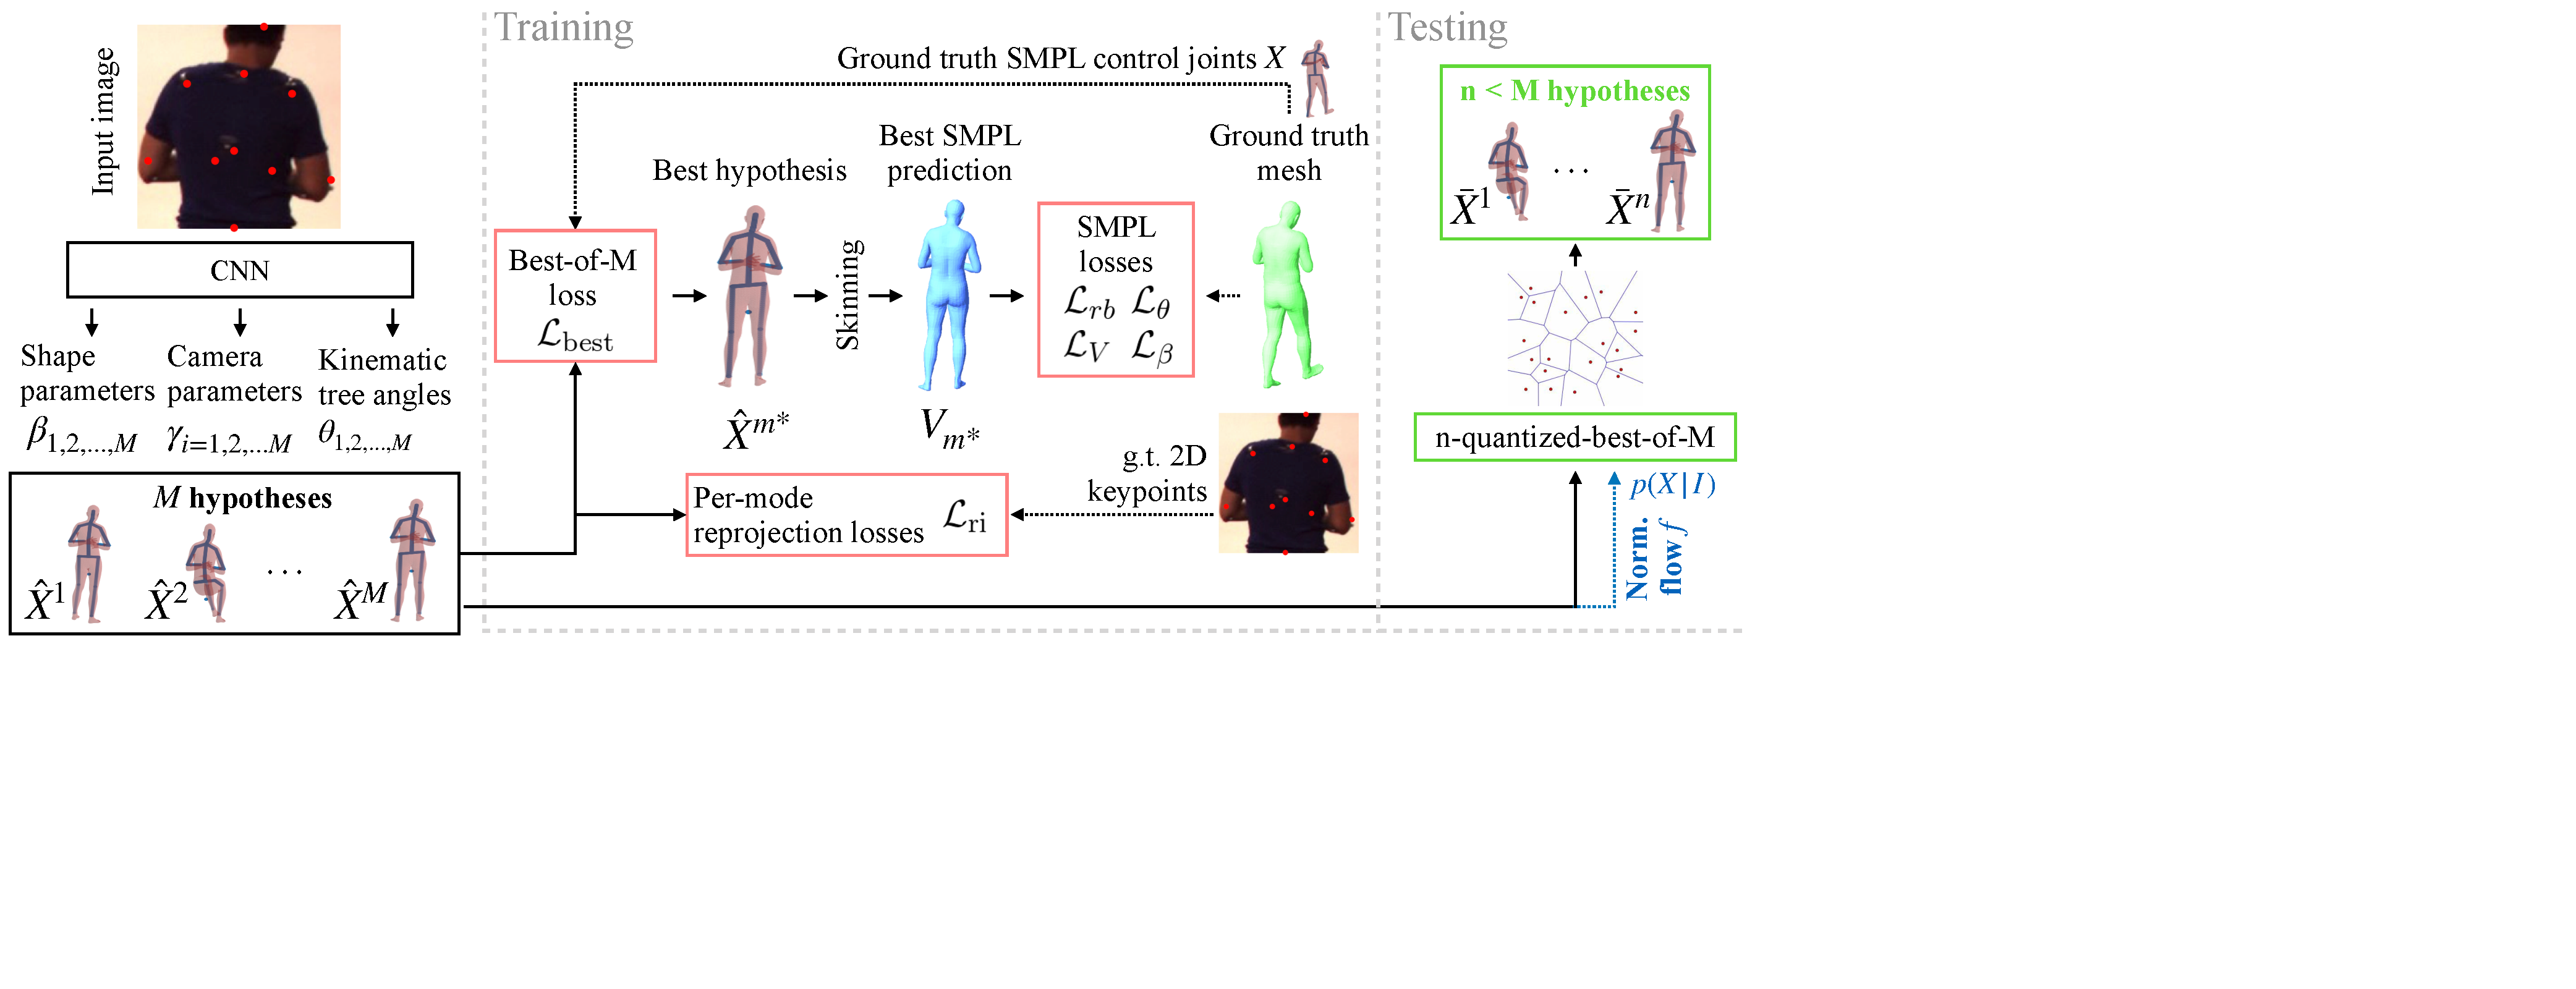
\includegraphics[width=\linewidth]{method/overview_v6.pdf}
\end{center}
\caption{\textbf{Overview of our method.}
Given a single image of a human, during training, our method produces multiple skeleton hypotheses $\{\hat Y^i\}_{i=1}^M$ that enter a Best-of-$M$ loss which selects the representative $\hat Y^{m^*}$ which most accurately matches the ground truth 3D control joints $Y$. 
% The camera parameters together with a skinned SMPL mesh enter the final set of SMPL losses.
At test time, we sample an arbitrary number of $n<M$ hypotheses by quantizing the set $\{\hat Y^i\}$ that is assumed to be sampled from the probability distribution $p(Y|I)$ modeled with normalizing flow $f$.
}\label{fig:arch_diagram}
\end{figure*}